% -*- mode: latex; mode: reftex; mode: outline-minor -*-
\documentclass[dvipdfmx]{jsarticle}
\usepackage{amsmath,amssymb}
\usepackage[dvipdfmx]{graphicx}
\usepackage{booktabs}
\usepackage{url}
\usepackage[framemethod=tikz]{mdframed}
\usepackage{fancyvrb}
\usepackage{color}
\newcommand{\R}{\color{red}}
\newcommand{\B}{\color{black}}
\newcommand{\E}{!}

\title{スキルシミュレータメーカーのチュートリアル
\\
{\small 1版. 2021年4月1日}
}
\date{}
\author{5chスキルシミュレータ開発Ver.13の480}

\begin{document}
\maketitle
\tableofcontents

\section{はじめに} %%%%%%%%%%%%%%%%
この文書はいわゆる「スキルシミュメーカー」%
\footnote{スキルシミュツクールでも良いですが、
ツクールがKADOKAWAの商標なのでやめました。}%
の利用方法のチュートリアルです。

\begin{itemize}
\item 
Cやjavascriptのプログラムは不要です。
\item 
独自言語でスキルシミュレータを記述します。
\item 
シミュレータの生成には、rubyの実行環境が必要ですが、
ウェブ上で生成できるページも用意してあります
(\url{http://nap.s3.xrea.com/simgen-demo.html})。
このデモは、入力ファイルサイズが大きいと動作しないかも知れません%
\footnote{%
サイズの目安としては、
モンスターハンターワールド:アイスボーンの装備やスキルの数であれば、
入力ファイルサイズは1万行を超えます。
プログラム不要といっても、この規模のテキストを手で作成することは
現実的ではないので、
何らかのプログラムで出力することにはなると思います。
それでも、1からシミュレータを作るよりは格段に易しいプログラムで済みます。
}。
\item 
モンスターハンターライズ専用ではないので、過去作品、将来の作品どころか、
別のゲームにも使えるかも知れません。
\end{itemize}

このチュートリアルでは、
シミュレータを生成するための独自言語の完全な仕様を説明することはせずに、
ごく簡単なシミュレータを生成するための入力ファイル (22行) から始めて、
徐々に複雑なもの (最後は78行) の例をもとに説明をします。
長くなりますが各段階で入力ファイル全文を掲載し、
説明は前段階にはなかった部分について行います。

シミュレータは線形計画法を用いたもので、
その原理を知りたい方は、
\url{https://github.com/13-480/lp-doc/blob/main/lpsim-v4.pdf}を参照して下さい。
よく見るシミュとは動作が違うのでこのチュートリアルの最後の方で補足します。

\section{最初のシミュ} %%%%%%%%%%%%%%%%
装備は、「フク」が2種類だけの簡単なスキルシミュレータの例を考えます。
スキル、珠、スロットはまだありません。
%
\begin{center}
\begin{tabular}{lr}
\toprule
フク       & 防御力 \\
\midrule
ポロシャツ & 1 \\
パーカー   & 2 \\
\bottomrule
\end{tabular}
\end{center}
%
入力ファイルは以下のようになります。
その後に内容の説明をします。
\medskip

{\footnotesize\begin{mdframed}\begin{Verbatim}
# チュートリアルその1
[META]
title チュートリアル1 (最初のシミュ)

[INDUCE]
ポロシャツ  ->  防御力  1
パーカー    ->  防御力  2

[RELATION]
ポロシャツ + パーカー <= 1

[UI]
(0..C) ポロシャツ
(0..C) パーカー

[QUERY]
検索 検索中止 追加検索 防御力

[SUMMARY]
v 防御力
n* ポロシャツ
n* パーカー
\end{Verbatim}
\end{mdframed}}

\subsection{入力ファイルの内容の説明}

\paragraph{コメント}~\medskip
{\footnotesize\begin{mdframed}\begin{Verbatim}
# チュートリアルその1
\end{Verbatim}
\end{mdframed}}
\medskip

「\texttt{\#}」以降行末まではコメントで、無視されます。

\paragraph{METAセクション}~\medskip
{\footnotesize\begin{mdframed}\begin{Verbatim}
[META]
title チュートリアル1 (最初のシミュ)
\end{Verbatim}
\end{mdframed}}
\medskip

titleで始まる行で、生成されるウェブページのタイトルを指定します。

\begin{center}
\frame{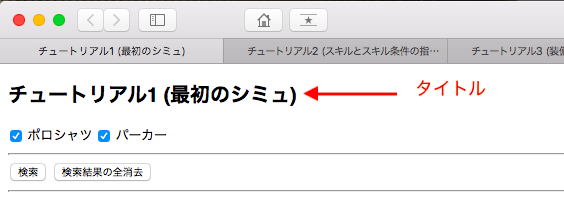
\includegraphics[scale=0.5]{./fig/fig00.png}}
\end{center}

\paragraph{INDUCEセクション}~\medskip
{\footnotesize\begin{mdframed}\begin{Verbatim}
[INDUCE]
ポロシャツ  ->  防御力  1
パーカー    ->  防御力  2
\end{Verbatim}
\end{mdframed}}
\medskip

各装備が、スキル、スロット、属性耐性等のパラメータを
どれだけ発動するかを指定します%
\footnote{
この例では、実際には、
「\texttt{防御力 = ポロシャツ + 2 パーカー」}
という式を、RELATIONセクションに指定するのと同じです。
RELATIONセクションだけで済むのにINDUCEセクションを設ける理由は、
現在2種類であるフクの種類が大量になった場合、この式が長大になってしまうので、
これを避けたいからです。
}。
この例では、ポロシャツの防御力が1、パーカーの防御力が2と指定しています。

\paragraph{RELATIONセクション}~\medskip
{\footnotesize\begin{mdframed}\begin{Verbatim}
[RELATION]
ポロシャツ + パーカー <= 1
\end{Verbatim}
\end{mdframed}}
\medskip

装備の数などの満たすべき関係式を指定します。
この例では、ポロシャツの装備数とパーカーの装備数の和が1以下であるという
指定です。
ポロシャツとパーカーのどちらか一方だけ1であるか、両方0だけが可能なので、
装備できるのはどちらか一方、
あるいは装備なしだけが可能であることを意味しています。

\paragraph{UIセクション}~\medskip
{\footnotesize\begin{mdframed}\begin{Verbatim}
[UI]
(0..C) ポロシャツ
(0..C) パーカー
\end{Verbatim}
\end{mdframed}}
\medskip

UIセクションでは、
装備の所持数等を設定するプルダウンメニュー、テキストボックス、
チェックボックスを、ブラウザ上にどう表示するかを指定します。

「\texttt{(0..C) ポロシャツ}」は、
ポロシャツ所持数の最小値が0で、
最大値はシミュレータ上に表示されるチェックボックスで指定されるという意味です。
チェックボックスはチェックされていれば1、いなければ0を表します。
数値が固定されていて、チェックボックス等で設定する必要のない
最小値の0に対応するものは、シミュレータに表示されません。

\begin{center}
\frame{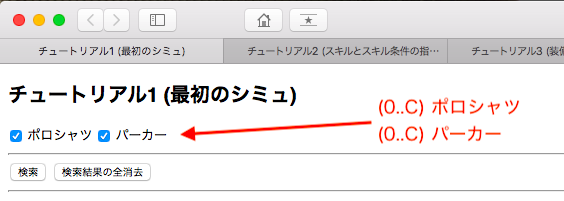
\includegraphics[scale=0.5]{./fig/fig01.png}}
\end{center}

\paragraph{QUERYセクション}~\medskip
{\footnotesize\begin{mdframed}\begin{Verbatim}
[QUERY]
検索 検索中止 追加検索 防御力
\end{Verbatim}
\end{mdframed}}
\medskip

検索ボタンは状態によって表示されるテキストが変わるので、それを指定します。
4つある文字列の最初の3つは、順に、
初期状態の表示文字列、検索中の表示文字列、
検索が終わって検索結果が画面に残っているときの表示文字列です。

4つある文字列の最後は、何を最大化して検索するかを指定します。
つまり、条件を満たすものたちのうち、防御力最大のものを検索するという指定です。

\begin{center}
\frame{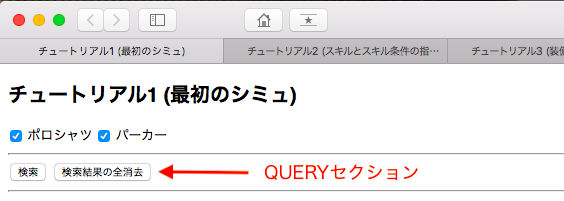
\includegraphics[scale=0.5]{./fig/fig02.png}}
\end{center}

\paragraph{SUMMARYセクション}~\medskip
{\footnotesize\begin{mdframed}\begin{Verbatim}
[SUMMARY]
v 防御力
n* ポロシャツ
n* パーカー
\end{Verbatim}
\end{mdframed}}
\medskip

検索結果として何を表示するか指定します。
正確には、検索結果の「見出し」部分の表示です。

この例では、防御力、ポロシャツ、パーカーについて、
合計3件の情報を表示します。
行頭の記号の意味は以下のとおりです。
%
\begin{center}
\begin{tabular}{cccc}
\toprule
記号 & \texttt{n} &\texttt{v} & \texttt{*} \\
\midrule
意味 & 名前を表示 & 値を表示 & 値が0なら何も表示しない \\
\bottomrule
\end{tabular}
\end{center}
%
従って、防御力はその値だけを表示し、
ポロシャツとパーカーは、0でなければ
(UIセクションでの指定により1であることが確定) 名前だけ表示します。

\begin{center}
\frame{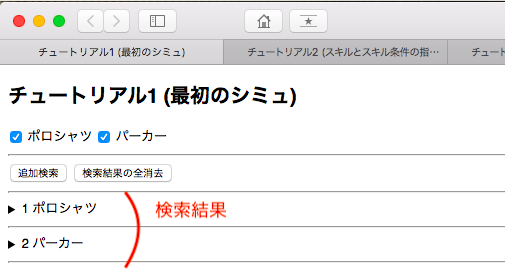
\includegraphics[scale=0.5]{./fig/fig03.png}}
\end{center}

\section{スキルとスキル条件の指定} %%%%%%%%%%%%%%%%
前節ではスキルがありませんでしたが、「攻撃」スキルを導入してみます。
珠、スロットはまだありません。

%
\begin{center}
\begin{tabular}{lrr}
\toprule
フク       & 防御力 & 攻撃スキル\\
\midrule
ポロシャツ & 1 & 1 \\
パーカー   & 2 & 0 \\
\bottomrule
\end{tabular}
\end{center}
%
入力ファイルの全体は以下のとおりで、
前節からの変更箇所を赤くしています。
入力ファイルの後に記す内容の説明は、変更のあった場所に限定します。
\medskip

{\footnotesize\begin{mdframed}\begin{Verbatim}[commandchars=!<>]
# チュートリアルその2
[META]
title チュートリアル2 (スキルとスキル条件の指定)

[INDUCE]
ポロシャツ  ->  防御力  1!R!-,  攻撃  1
パーカー    ->  防御力  2

[RELATION]
ポロシャツ + パーカー <= 1

[UI] !R!-width:150px
(0..C) ポロシャツ
(0..C) パーカー
!R!-[UI] br
!R!-([0 1 2 3 4 5]..5) 攻撃
!R!-(0?..) 防御力

[QUERY]
検索 検索中止 追加検索 防御力

[SUMMARY]
v 防御力
n* ポロシャツ
n* パーカー

!R!-[DETAILS] newrow
!R!-[DETAILS] スキル
!R!-nv* 攻撃
\end{Verbatim}
\end{mdframed}}

\subsection{入力ファイルの内容の説明}

\paragraph{INDUCEセクション}~\medskip
{\footnotesize\begin{mdframed}\begin{Verbatim}[commandchars=!<>]
[INDUCE]
ポロシャツ  ->  防御力  1!R!-,  攻撃  1
パーカー    ->  防御力  2
\end{Verbatim}
\end{mdframed}}
\medskip

ポロシャツが攻撃Lv1を発動するので、ポロシャツの行に攻撃スキルの指定を
追加します。
このように、複数のものを発動するときは、カンマ区切りで記述します。

\paragraph{UIセクション}~\medskip
{\footnotesize\begin{mdframed}\begin{Verbatim}[commandchars=!<>]
[UI] !R!-width:150px
(0..C) ポロシャツ
(0..C) パーカー
!R!-[UI] br
!R!-([0 1 2 3 4 5]..5) 攻撃
!R!-(0?..) 防御力
\end{Verbatim}
\end{mdframed}}
\medskip

「\texttt{[UI] width:150px}」は、UI部品の幅を指定します。
この指定により、UI部品をきれいに揃えることができます。
指定を解除するには 「\texttt{[UI] nowidth}」 と記述します。

「\texttt{[UI] br}」は改行です。
次のUI部品は、新しい行から表示されます。

「\texttt{([0 1 2 3 4 5]..5) 攻撃}」
の最小値の部分は、0から5までを選択できるプルダウンメニューを表しています。
ポロシャツと同様の指定ですが、プルダウンが最小値の方に付きます。
これにより、「攻撃スキルが2以上」などの条件指定が可能になります。
ただし、シミュレータでの表示だけを見ても、
最小値の指定か最大値の指定かは区別できませんので、
文脈でわかるようにUI部品を配置する必要があります。

「\texttt{(0?..) 防御力}」
の最小値の部分のように、数値の後に「?」を付けると、
値をテキストボックスで入力できるようになります。
この場合の「0」はテキストボックスの初期値です。
また、最大値の記載がありませんが、その場合は上限なしとなります。

\begin{center}
\frame{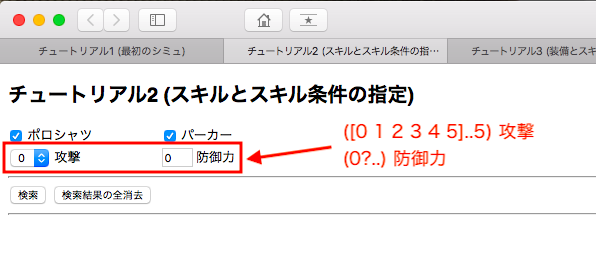
\includegraphics[scale=0.5]{./fig/fig04.png}}
\end{center}

\paragraph{DETAILSセクション}~\medskip
{\footnotesize\begin{mdframed}\begin{Verbatim}[commandchars=!<>]
!R!-[DETAILS] newrow
!R!-[DETAILS] スキル
!R!-nv* 攻撃
\end{Verbatim}
\end{mdframed}}
\medskip

先の例の検索結果表示は、
検索結果の「見出し」部分の表示を指定するSUMMARYセクションのみでした。
「見出し」部分をクリックすると、折りたたまれている「詳細」部分が現れますが、
DETAILSセクションでは、「詳細」部分の表示を指定します。

詳細部分は、段組表示が基本で、
「\texttt{[DETAILS] newrow}」は新しい段の開始です。

「\texttt{[DETAILS] スキル}」はその段の1行目に表示する文字列の指定です%
\footnote{
1行目でなくても任意の位置で文字列の表示が可能です
}。

「\texttt{nv* 攻撃}」はSUMMARYセクションと同じで、
値が0でないときに限り、攻撃の名前と値を表示します。

\begin{center}
\frame{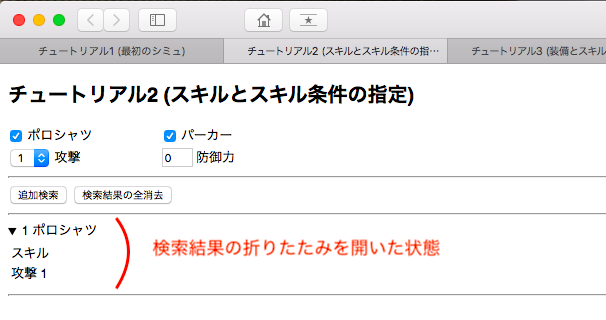
\includegraphics[scale=0.5]{./fig/fig05.png}}
\end{center}

\section{装備とスキルの種類が増えた場合の工夫} %%%%%%%%%%%%%%%%
前節では装備が2種類、スキルが1種類でしたが、これらを増やしてみます。
種類が増えても、関係式が長くならないような書き方、
見辛くならないような表示の体裁の指定の仕方を説明します。
%
珠、スロットはまだありません。
%
\begin{center}
\begin{tabular}{llrrrr}
\toprule
&& 防御力 & 攻撃スキル & 解放スキル\\
\midrule
フク
& ポロシャツ & 1 & 1 & 0\\
& パーカー   & 2 & 0 & 0\\
\midrule
クツ
& サンダル & 1 & 0 & 0\\
& スリッパ & 2 & 0 & 1\\
\bottomrule
\end{tabular}
\end{center}
%
入力ファイルの全体は以下のとおりで、
前節からの変更箇所を赤くしています。
入力ファイルの後に記す内容の説明は、変更のあった場所に限定します。
\medskip

{\footnotesize\begin{mdframed}\begin{Verbatim}[commandchars=!<>]
# チュートリアルその3
[META]
title チュートリアル3 (装備とスキルの種類が増えた場合の工夫)

[INDUCE]
!R!-フクなし    ->                        フク  1   
ポロシャツ  ->  防御力  1,  攻撃  1!R!-,  フク  1
パーカー    ->  防御力  2!R!-,            フク  1
                                   
!R!-クツなし    ->                        クツ  1
!R!-サンダル    ->  防御力  1,            クツ  1
!R!-スリッパ    ->  防御力  2,  解放  1,  クツ  1

[RELATION]
!R!-フク = クツ = 1

[UI] width:150px
!R!-[UI] subsection フク
!R!-(0..1) フクなし
(0..C) ポロシャツ
(0..C) パーカー

!R!-[UI] subsection クツ
!R!-(0..1) クツなし
!R!-(0..C) サンダル
!R!-(0..C) スリッパ

!R!-[UI] subsection スキル条件・最低防御力指定
([0 1 2 3 4 5]..5) 攻撃
!R!-([0 1 2 3]..3) 解放
(0?..) 防御力

[QUERY]
検索 検索中止 追加検索 防御力

[SUMMARY] !R!-width:50px
v 防御力
!R!-[SUMMARY] width:150px
!R!-n* フクなし
n* ポロシャツ
n* パーカー
!R!-n* クツなし
!R!-n* サンダル
!R!-n* スリッパ

[DETAILS] newrow
[DETAILS] スキル
nv* 攻撃
!R!-nv* 解放
\end{Verbatim}
\end{mdframed}}

\subsection{入力ファイルの内容の説明}

\paragraph{INDUCEセクション、RELATIONセクション}~\medskip
{\footnotesize\begin{mdframed}\begin{Verbatim}[commandchars=!<>]
[INDUCE]
!R!-フクなし    ->                        フク  1   
ポロシャツ  ->  防御力  1,  攻撃  1!R!-,  フク  1
パーカー    ->  防御力  2!R!-,            フク  1
                                   
!R!-クツなし    ->                        クツ  1
!R!-サンダル    ->  防御力  1,            クツ  1
!R!-スリッパ    ->  防御力  2,  解放  1,  クツ  1

[RELATION]
!R!-フク = クツ = 1
\end{Verbatim}
\end{mdframed}}
\medskip

サンダルとスリッパが増えた分と、
スリッパに付いている解放スキルの分を追記してあります。

「フク」については、「\texttt{フク = フクなし + ポロシャツ + パーカー}」
が生成されます。
そして、RELATIONセクションに「\texttt{フク = 1}」とあるので、
結局、「\texttt{フクなし + ポロシャツ + パーカー = 1}」
が生成されていることになります%
\footnote{
これを直にRELATIONセクションに書いても良いですが、
装備の数が増えたときに長大な式になるので、INDUCEセクションを利用しています。
}。

また「フクなし」という、何も選ばない状態を表す、
実際にはない装備を導入しています。
RELATIONセクションで
「\texttt{フク <= 1}」ではなく「\texttt{フク = 1}」としたことで%
\footnote{
RELATIONセクションには、3つ以上であっても、複数の式を、
\texttt{=}、\texttt{<=}、\texttt{>=}
でつないだ式を書けます。
}、
どれか1つは必ず1になるので、
ポロシャツもパーカーも0のときはフクなしが1になり、
その場合SUMMARYセクションに何も表示されないのではなく、
「フクなし」と表示させることができます。
%
「クツなし」も同様です。

\paragraph{UIセクション}~\medskip
{\footnotesize\begin{mdframed}\begin{Verbatim}[commandchars=!<>]
[UI] width:150px
!R!-[UI] subsection フク
!R!-(0..1) フクなし
(0..C) ポロシャツ
(0..C) パーカー

!R!-[UI] subsection クツ
!R!-(0..1) クツなし
!R!-(0..C) サンダル
!R!-(0..C) スリッパ

!R!-[UI] subsection スキル条件・最低防御力指定
([0 1 2 3 4 5]..5) 攻撃
!R!-([0 1 2 3]..3) 解放
(0?..) 防御力
\end{Verbatim}
\end{mdframed}}
\medskip

「\texttt{[UI] subsection フク}」
は、「フク」を見出しにした、折りたたみ可能な部品で出力する指定です。
装備が大量になったときは、必要なもの以外は折りたたむことを可能にします%
\footnote{
よく見るスキルシミュレータでは、
頭・胴・腕・腰・脚の5部位が横に並ぶようにするなど、
防具のシリーズごとに分類しています。
この例では練習のためフクとクツで分類しましたが、
よく見るものにならうと、
subsection「よそいき」にポロシャツとサンダルを置き、
subsection「部屋着」にパーカーとスリッパを置くなどとなります。
}。

「\texttt{(0..1) フクなし}」は、最小値・最大値とも定数ですので、
UI部品が生成されません。
つまり、RELATIONセクションに「\texttt{0 <= フクなし <= 1}」
と記述するのと同じです。「クツなし」も同様です。

攻撃スキルの最大レベルは5にしていましたが、
新設の解放スキルの最大は3としました。

\begin{center}
\frame{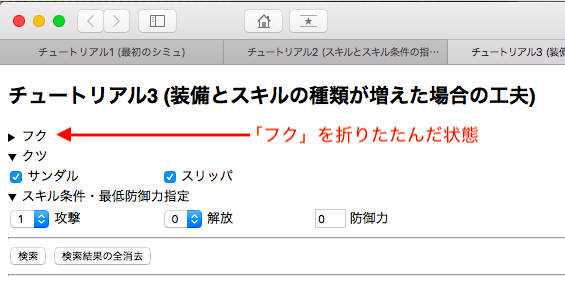
\includegraphics[scale=0.5]{./fig/fig06.png}}
\end{center}

\paragraph{SUMMARYセクション}~\medskip
{\footnotesize\begin{mdframed}\begin{Verbatim}[commandchars=!<>]
[SUMMARY] !R!-width:50px
v 防御力
!R!-[SUMMARY] width:150px
!R!-n* フクなし
n* ポロシャツ
n* パーカー
!R!-n* クツなし
!R!-n* サンダル
!R!-n* スリッパ
\end{Verbatim}
\end{mdframed}}
\medskip

UIセクションと同様に、SUMMARYセクションでも
「\texttt{[SUMMARY] width:50px}」のように、
表示される部品の幅を指定できます。
これにより、検索結果が複数表示されているときも、
表示が揃うようになります。

\begin{center}
\frame{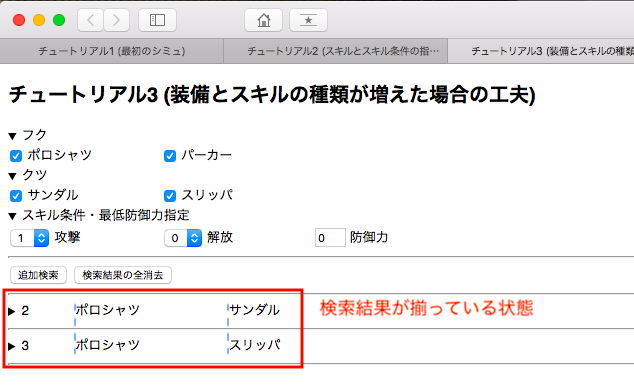
\includegraphics[scale=0.5]{./fig/fig07.png}}
\end{center}

\paragraph{DETAILSセクション}~\medskip
{\footnotesize\begin{mdframed}\begin{Verbatim}[commandchars=!<>]
[DETAILS] newrow
[DETAILS] スキル
nv* 攻撃
!R!-nv* 解放
\end{Verbatim}
\end{mdframed}}
\medskip

攻撃と同様に解放スキルも表示させます。

\section{スロットと珠} %%%%%%%%%%%%%%%%
防具に「スロット」があり、そこにスキルを持った「珠」を装着できる
ことを考えてみます。
%
このチュートリアルでは最終的には大・中・小3種類のスロットを
考えますが、この節では小スロットのみを考え、
次節で3種類のスロットを考えることにします。
%
以下、入力ファイルでは、小スロットを短く「小スロ」と表します。
%
\begin{center}
\begin{tabular}{llrrrrr}
\toprule
&& 防御力 & 攻撃スキル & 解放スキル & 小スロット\\
\midrule
フク
& ポロシャツ & 1 & 1 & 0 & 0\\
& パーカー   & 2 & 0 & 0 & 2\\
\midrule
クツ
& サンダル & 1 & 0 & 0 & 0\\
& スリッパ & 2 & 0 & 1 & 1\\
\bottomrule
\end{tabular}
\end{center}
%
\begin{center}
\begin{tabular}{llrrrrr}
\toprule
珠 & スキル & 必要スロット \\
\midrule
攻撃珠 & 攻撃1 & 小\\
\bottomrule
\end{tabular}
\end{center}
%
入力ファイルの全体は以下のとおりで、
前節からの変更箇所を赤くしています。
入力ファイルの後に記す内容の説明は、変更のあった場所に限定します。
\medskip

{\footnotesize\begin{mdframed}\begin{Verbatim}[commandchars=!<>]
# チュートリアルその4
[META]
title チュートリアル4 (スロットと珠)

[INDUCE]
フクなし    ->                        フク  1   
ポロシャツ  ->  防御力  1,  攻撃  1,  フク  1
パーカー    ->  防御力  2,            フク  1!R!-,  小スロ 2
                                   
クツなし    ->                        クツ  1
サンダル    ->  防御力  1,            クツ  1
スリッパ    ->  防御力  2,  解放  1,  クツ  1!R!-,  小スロ 1

!R!-攻撃珠  ->  攻撃  1,  小スロ  -1

[RELATION]
フク = クツ = 1
!R!-小スロ >= 0

[UI] width:150px
[UI] subsection フク
(0..1) フクなし
(0..C) ポロシャツ
(0..C) パーカー

[UI] subsection クツ
(0..1) クツなし
(0..C) サンダル
(0..C) スリッパ

!R!-[UI] subsection 珠
!R!-(0..[0 1 2 3 4 5]) 攻撃珠

[UI] subsection スキル条件・最低防御力指定
([0 1 2 3 4 5]..5) 攻撃
([0 1 2 3]..3) 解放
(0?..) 防御力

[QUERY]
検索 検索中止 追加検索 防御力

[SUMMARY] width:50px
v 防御力
[SUMMARY] width:150px
n* フクなし
n* ポロシャツ
n* パーカー
n* クツなし
n* サンダル
n* スリッパ

[DETAILS] newrow
[DETAILS] スキル
nv* 攻撃
nv* 解放

!R!-[DETAILS] newrow
!R!-[DETAILS] 珠
!R!-nv* 攻撃珠

!R!-[DETAILS] newrow
!R!-[DETAILS] 空きスロット
!R!-nv 小スロ 
\end{Verbatim}
\end{mdframed}}

\subsection{入力ファイルの内容の説明}

\paragraph{INDUCEセクション}~\medskip
{\footnotesize\begin{mdframed}\begin{Verbatim}[commandchars=!<>]
[INDUCE]
フクなし    ->                        フク  1   
ポロシャツ  ->  防御力  1,  攻撃  1,  フク  1
パーカー    ->  防御力  2,            フク  1!R!-,  小スロ 2
                                   
クツなし    ->                        クツ  1
サンダル    ->  防御力  1,            クツ  1
スリッパ    ->  防御力  2,  解放  1,  クツ  1!R!-,  小スロ 1

!R!-攻撃珠  ->  攻撃  1,  小スロ  -1
\end{Verbatim}
\end{mdframed}}
\medskip

パーカーが小スロットを2つ、スリッパが小スロットを1つ発動することを指定します。

また、攻撃珠が攻撃のスキルレベルを1発動し、
小スロット1つを消費することも指定します。
消費する場合は負の値になります。

\paragraph{RELATIONセクション}~\medskip
{\footnotesize\begin{mdframed}\begin{Verbatim}[commandchars=!<>]
[RELATION]
フク = クツ = 1
!R!-小スロ >= 0
\end{Verbatim}
\end{mdframed}}
\medskip

珠が小スロットに装着できるには、珠が必要とする小スロット数が、
防具に備わっている小スロット数以下である必要があります。
INDUCEセクションで、珠の消費する小スロット数を負で与えていますので、
小スロの値は、消費されずに残っているスロット数です。
従って、条件は「\texttt{小スロ >= 0}」と表せることになります。

\paragraph{UIセクション}~\medskip
{\footnotesize\begin{mdframed}\begin{Verbatim}[commandchars=!<>]
[UI] width:150px

(中略)

!R!-[UI] subsection 珠
!R!-(0..[0 1 2 3 4 5]) 攻撃珠

(攻略)
\end{Verbatim}
\end{mdframed}}
\medskip

珠の所持数の設定も指定します。

\begin{center}
\frame{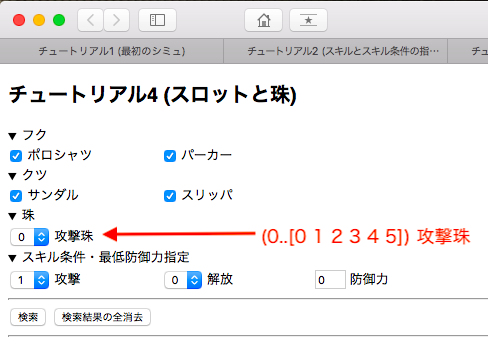
\includegraphics[scale=0.5]{./fig/fig08.png}}
\end{center}

\paragraph{DETAILSセクション}~\medskip
{\footnotesize\begin{mdframed}\begin{Verbatim}[commandchars=!<>]
[DETAILS] newrow
[DETAILS] スキル
nv* 攻撃
nv* 解放

!R!-[DETAILS] newrow
!R!-[DETAILS] 珠
!R!-nv* 攻撃珠

!R!-[DETAILS] newrow
!R!-[DETAILS] 空きスロット
!R!-nv 小スロ 
\end{Verbatim}
\end{mdframed}}
\medskip

結果表示の詳細部分に、
珠の個数と空きスロットを、ともに1列設けて表示します。

\begin{center}
\frame{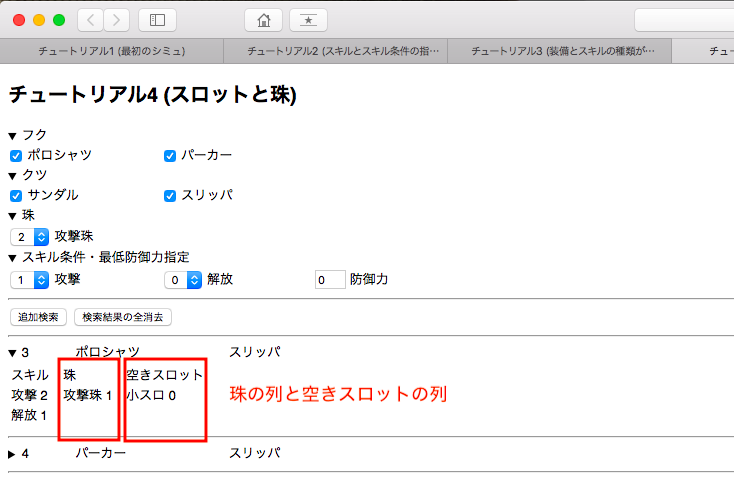
\includegraphics[scale=0.5]{./fig/fig09.png}}
\end{center}

\section{大きさの違うスロット} %%%%%%%%%%%%%%%%
前節では小スロットだけでしたが、この節では大・中・小3種類のスロットを考えます。
鍵は、RELATIONセクションの関係式ですが、なぜそうなるかは省きます。
\url{https://github.com/13-480/lp-doc/blob/main/lpsim-v4.pdf}に説明があります。

スキルシミュメーカの現在のバージョンでは、
大・中・小のスロットそれぞれの空き数を得られず、
大きさを無視した合計スロット数だけが得られます。
スロットの空きが1次式で表せないのが理由で、
現時点では入力ファイルを工夫するだけでは不可能です。

新たに、ポロシャツにスロットを4つ追加し、
攻撃大珠も新設しました。
\medskip
%
\begin{center}
\begin{tabular}{llrrrrrrr}
\toprule
&& 防御力 & 攻撃スキル & 解放スキル & 小スロット& 中スロット& 大スロット\\
\midrule
フク
& ポロシャツ & 1 & 1 & 0 & 2 & 1 & 1\\
& パーカー   & 2 & 0 & 0 & 2 & 0 & 0\\
\midrule
クツ
& サンダル & 1 & 0 & 0 & 0 & 0 & 0\\
& スリッパ & 2 & 0 & 1 & 1 & 0 & 0\\
\bottomrule
\end{tabular}
\end{center}
%
\begin{center}
\begin{tabular}{llrrrrr}
\toprule
珠 & スキル & 必要スロット \\
\midrule
攻撃珠 & 攻撃1 & 小\\
攻撃大珠 & 攻撃2 & 大\\
\bottomrule
\end{tabular}
\end{center}
%
入力ファイルの全体は以下のとおりで、
前節からの変更箇所を赤くしています。
入力ファイルの後に記す内容の説明は、変更のあった場所に限定します。
\medskip

{\footnotesize\begin{mdframed}\begin{Verbatim}[commandchars=!<>]
# チュートリアルその5
[META]
title チュートリアル5 (大きさの違うスロット)

[INDUCE]
フクなし    ->                        フク  1   
ポロシャツ  ->  防御力  1,  攻撃  1,  フク  1!R!-,  小スロ 2, 中スロ 1, 大スロ 1
パーカー    ->  防御力  2,            フク  1,  小スロ 2
                                   
クツなし    ->                        クツ  1
サンダル    ->  防御力  1,            クツ  1
スリッパ    ->  防御力  2,  解放  1,  クツ  1,  小スロ 1

攻撃珠    ->  攻撃  1,  小スロ  -1
!R!-攻撃大珠  ->  攻撃  2,  大スロ  -1

[RELATION]
フク = クツ = 1
!R!-大スロ >= 0
!R!-大スロ + 中スロ >= 0
!R!-大スロ + 中スロ + 小スロ >= 0
!R!-空きスロット合計 = 大スロ + 中スロ + 小スロ

[UI] width:150px
[UI] subsection フク
(0..1) フクなし
(0..C) ポロシャツ
(0..C) パーカー

[UI] subsection クツ
(0..1) クツなし
(0..C) サンダル
(0..C) スリッパ

[UI] subsection 珠
(0..[0 1 2 3 4 5]) 攻撃珠
!R!-(0..[0 1 2]) 攻撃大珠

[UI] subsection スキル条件・最低防御力指定
([0 1 2 3 4 5]..5) 攻撃
([0 1 2 3]..3) 解放
(0?..) 防御力

[QUERY]
検索 検索中止 追加検索 防御力

[SUMMARY] width:50px
v 防御力
[SUMMARY] width:150px
n* フクなし
n* ポロシャツ
n* パーカー
n* クツなし
n* サンダル
n* スリッパ

[DETAILS] newrow
[DETAILS] スキル
nv* 攻撃
nv* 解放

[DETAILS] newrow
[DETAILS] 珠
nv* 攻撃珠
!R!-nv* 攻撃大珠

[DETAILS] newrow
[DETAILS] 空きスロット
!R!-nv 空きスロット合計
\end{Verbatim}
\end{mdframed}}

\subsection{入力ファイルの内容の説明}

\paragraph{INDUCEセクション}~\medskip
{\footnotesize\begin{mdframed}\begin{Verbatim}[commandchars=!<>]
[INDUCE]
フクなし    ->                        フク  1   
ポロシャツ  ->  防御力  1,  攻撃  1,  フク  1!R!-,  小スロ 2, 中スロ 1, 大スロ 1
パーカー    ->  防御力  2,            フク  1,  小スロ 2
                                   
(中略)

攻撃珠    ->  攻撃  1,  小スロ  -1
!R!-攻撃大珠  ->  攻撃  2,  大スロ  -1
\end{Verbatim}
\end{mdframed}}
\medskip

ポロシャツにスロットを追加し、攻撃大珠を新設します。

\paragraph{RELATIONセクション}~\medskip
{\footnotesize\begin{mdframed}\begin{Verbatim}[commandchars=!<>]
[RELATION]
フク = クツ = 1
!R!-大スロ >= 0
!R!-大スロ + 中スロ >= 0
!R!-大スロ + 中スロ + 小スロ >= 0
!R!-空きスロット合計 = 大スロ + 中スロ + 小スロ
\end{Verbatim}
\end{mdframed}}
\medskip

スロットに関する関係式は、「\texttt{小スロ >= 0}」などとはならないです。
このチュートリアルでは説明は省きます。

ただし、
「\texttt{大スロ + 中スロ + 小スロ}」は、空きスロット
合計に一致するので、これだけは利用することにします。

\paragraph{UIセクション}~\medskip
{\footnotesize\begin{mdframed}\begin{Verbatim}[commandchars=!<>]
[UI] width:150px

(中略)

[UI] subsection 珠
(0..[0 1 2 3 4 5]) 攻撃珠
!R!-(0..[0 1 2]) 攻撃大珠

(攻略)
\end{Verbatim}
\end{mdframed}}
\medskip

攻撃大珠の所持数指定を追加します。

\paragraph{DETAILSセクション}~\medskip
{\footnotesize\begin{mdframed}\begin{Verbatim}[commandchars=!<>]
[DETAILS] newrow

(中略)

[DETAILS] newrow
[DETAILS] 珠
nv* 攻撃珠
!R!-nv* 攻撃大珠

[DETAILS] newrow
[DETAILS] 空きスロット
!R!-nv 空きスロット合計
\end{Verbatim}
\end{mdframed}}
\medskip

攻撃大珠と空きスロットの表示を追加します。

\section{スキルレベル上限解放、結果表示の工夫} %%%%%%%%%%%%%%%%
ここでは、モンスターハンターワールド:アイスボーンで
言うところの極意、つまり、
スキルレベルの上限解放を説明します。

また、スキルの種類が増えた場合の、
検索対象のスキルと、そうではないがおまけで付いてきたスキルを
区別して表示する方法も説明します。
\medskip
%
\begin{center}
\begin{tabular}{llrrrrrrr}
\toprule
&& 防御力 & 攻撃スキル & 解放スキル & 小スロット& 中スロット& 大スロット\\
\midrule
フク
& ポロシャツ & 1 & 1 & 0 & 2 & 1 & 1\\
& パーカー   & 2 & 0 & 0 & 2 & 0 & 0\\
\midrule
クツ
& サンダル & 1 & 0 & 0 & 0 & 0 & 0\\
& スリッパ & 2 & 0 & 1 & 1 & 0 & 0\\
\bottomrule
\end{tabular}
\end{center}
%
\begin{center}
\begin{tabular}{llrrrrr}
\toprule
珠 & スキル & 必要スロット \\
\midrule
攻撃珠 & 攻撃1 & 小\\
攻撃大珠 & 攻撃2 & 大\\
解放珠 & 解放1 & 中\\
\bottomrule
\end{tabular}
\end{center}
%
入力ファイルの全体は以下のとおりで、
前節からの変更箇所を赤くしています。
入力ファイルの後に記す内容の説明は、変更のあった場所に限定します。
\medskip

{\footnotesize\begin{mdframed}\begin{Verbatim}[commandchars=!<>]
# チュートリアルその6
[META]
title チュートリアル6 (スキルレベル上限解放、結果表示の工夫)

[INDUCE]
フクなし    ->                        フク  1   
ポロシャツ  ->  防御力  1,  攻撃  1,  フク  1,  小スロ 2, 中スロ 1, 大スロ 1
パーカー    ->  防御力  2,            フク  1,  小スロ 2
                                   
クツなし    ->                        クツ  1
サンダル    ->  防御力  1,            クツ  1
スリッパ    ->  防御力  2,  解放  1,  クツ  1,  小スロ 1

攻撃珠    ->  攻撃  1,  小スロ  -1
攻撃大珠  ->  攻撃  2,  大スロ  -1
!R!-解放珠    ->  解放  1,  中スロ  -1

[RELATION]
フク = クツ = 1
大スロ >= 0
大スロ + 中スロ >= 0
大スロ + 中スロ + 小スロ >= 0
空きスロット合計 = 大スロ + 中スロ + 小スロ

!R!-[UNLOCK]
!R!-解放 3, 攻撃 3 5

[UI] width:150px
[UI] subsection フク
(0..1) フクなし
(0..C) ポロシャツ
(0..C) パーカー

[UI] subsection クツ
(0..1) クツなし
(0..C) サンダル
(0..C) スリッパ

[UI] subsection 珠
(0..[0 1 2 3 4 5]) 攻撃珠
(0..[0 1 2]) 攻撃大珠
!R!-(0..[0 1 2 3]) 解放珠

[UI] subsection スキル条件・最低防御力指定
([0 1 2 3 4 5]..5)!R!-* !B!-攻撃
([0 1 2 3]..3)!R!-* !B!-解放
(0?..) 防御力

[QUERY]
検索 検索中止 追加検索 防御力

[SUMMARY] width:50px
v 防御力
[SUMMARY] width:150px
n* フクなし
n* ポロシャツ
n* パーカー
n* クツなし
n* サンダル
n* スリッパ

[DETAILS] newrow
[DETAILS] !R!-検索対象スキル
nv* 攻撃
nv* 解放

!R!-[DETAILS] newrow
!R!-[DETAILS] !E!-対象外スキル

[DETAILS] newrow
[DETAILS] 珠
nv* 攻撃珠
nv* 攻撃大珠
!R!-nv* 解放珠

[DETAILS] newrow
[DETAILS] 空きスロット
nv 空きスロット合計
\end{Verbatim}
\end{mdframed}}


\subsection{入力ファイルの内容の説明}

\paragraph{INDUCEセクション}~\medskip
{\footnotesize\begin{mdframed}\begin{Verbatim}[commandchars=!<>]
[INDUCE]

(中略)

攻撃珠    ->  攻撃  1,  小スロ  -1
攻撃大珠  ->  攻撃  2,  大スロ  -1
!R!-解放珠    ->  解放  1,  中スロ  -1
\end{Verbatim}
\end{mdframed}}
\medskip

解放珠を新設します。

\paragraph{UNLOCKセクション}~\medskip
{\footnotesize\begin{mdframed}\begin{Verbatim}[commandchars=!<>]
!R!-[UNLOCK]
!R!-解放 3, 攻撃 3 5
\end{Verbatim}
\end{mdframed}}
\medskip

上限解放は上のように記述します。
この例では、解放スキルが3未満ならば攻撃スキルの上限は3、
解放スキルが3以上ならば攻撃スキルの上限は5と指定しています。

この指定を用いると、
攻撃スキルが3より高いものを検索したい時に、
解放スキルを3にする設定を手動でしていなくとも、
必ず解放スキルが3以上になる結果のみが得られます。




\paragraph{UIセクション}~\medskip
{\footnotesize\begin{mdframed}\begin{Verbatim}[commandchars=!<>]
[UI] width:150px

(中略)

[UI] subsection 珠
(0..[0 1 2 3 4 5]) 攻撃珠
(0..[0 1 2]) 攻撃大珠
!R!-(0..[0 1 2 3]) 解放珠

[UI] subsection スキル条件・最低防御力指定
([0 1 2 3 4 5]..5)!R!-* !B!-攻撃
([0 1 2 3]..3)!R!-* !B!-解放
(0?..) 防御力
\end{Verbatim}
\end{mdframed}}
\medskip

解放珠の所持数の設定を新設します。

また、「\texttt{([0 1 2 3 4 5]..5)* 攻撃}」と、
スキルレベル指定のうしろに「\texttt{*}」を付けると、
検索結果の表示で違いがあります。
%
「\texttt{*}」が付いていて、かつ、
そのスキルを検索してはいなかったとき、
つまり、上の攻撃スキルの例だと、プルダウンで0を選択していたとき%
\footnote{
正確には、最小値、最大値がプルダウンメニュー等で設定できる場合、
最小値は最も小さく、最大値は最も大きく設定されている場合が、
「検索していない」状態としています。
}、
本来表示すべき列の次の列に表示します。

これにより、検索対象スキルとおまけで付いてきたスキルを区別して
検索結果に表示することができます。

\paragraph{DETAILSセクション}~\medskip
{\footnotesize\begin{mdframed}\begin{Verbatim}[commandchars=!<>]
[DETAILS] newrow
[DETAILS] !R!-検索対象スキル
nv* 攻撃
nv* 解放

!R!-[DETAILS] newrow
!R!-[DETAILS] !E!-対象外スキル

[DETAILS] newrow
[DETAILS] 珠
nv* 攻撃珠
nv* 攻撃大珠
!R!-nv* 解放珠

[DETAILS] newrow
[DETAILS] 空きスロット
nv 空きスロット合計
\end{Verbatim}
\end{mdframed}}
\medskip

検索対象スキルの列の次に対象外スキルの列を追加しておきます。
中身は空ですが、UIセクションで「\texttt{*}」指定があれば、
この列に表示されることになります。

また、「\texttt{[DETAILS] !対象外スキル}」
のように、文字列先頭に「!」がある場合は、
既に前の列から移動してきたものがあっても、1行目に表示します。

\begin{center}
\frame{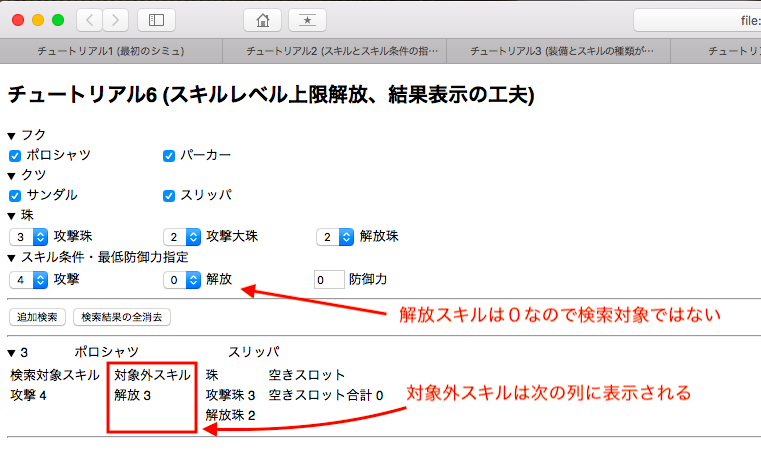
\includegraphics[scale=0.5]{./fig/fig10.png}}
\end{center}

\section{雑多な補足} %%%%%%%%%%%%%%%%

\subsection{ワンセット防具}
例えば、ポロシャツとサンダルはばらばらに装備することはできず、
常に同時に装備することしかできない場合
(モンスターハンターワールドのワンセット防具に相当)、
RELATIONセクションに
\medskip
\\
{\footnotesize\begin{mdframed}\begin{Verbatim}[commandchars=!<>]
[RELATION]
ポロシャツ = サンダル
\end{Verbatim}
\end{mdframed}}
\medskip
\noindent
と記述するとよいです (同時に0か、同時に1の可能性しかなくなるので)。
装備の部位がが2つより大きい場合も、
「\texttt{ポロシャツ = サンダル = メガネ}」
のようにするとよいです。

\subsection{検索結果が少ないこと (線形計画法)}
このツールで生成されるシミュレータの探索部分には、線形計画法が使われています。
ゲームが異なってもシミュレータには共通する部分がありますが、
高速化については個別の工夫がなされていました。
これを、線形計画法のライブラリに丸投げすることで、
高速化はすべてライブラリに任せることができるというメリットがあります。

よく見るシミュレータでは、条件に合致するものがある程度少なければ、
すべてを検索結果として表示します。
しかし、線形計画法のライブラリは、通常、条件に合致するもののうち、
例えば防御力最大のものを1つ結果として返します。
つまり、すべてを結果として表示しません。
このツールで生成されたシミュレータで検索を実行したとき、
1つしか検索結果が表示されない%
\footnote{
実際には、既存のライブラリ
「glpk.js」(\url{https://github.com/hgourvest/glpk.js})
に手を入れて、最良のものを発見する過程で見付かった、
最良ではない結果も表示できるようにしているので、
場合によっては2つ以上の結果が表示されることがあります。
\par
従って、1回目の検索でA、2回目でBとC、3回目でDが見付かり、
検索結果エリアにA、B、C、Dの順に並んだときでも、
防御力の大きい順とは限らないです。
$\rm{A} \geqq \rm{B} \geqq \rm{D}$ と
$\rm{B} \geqq \rm{C}$ は保証されますが、
CとDの大小は不明です。
}%
のはこれが理由です。

すべての結果を得たいときは、
既に見付かった装備の組合せを除外して、もう一度検索をして、
1つずつ見付ければよいです。
これが、「追加検索」ボタンの役割です。

\subsection{追加検索の条件}
その「追加検索」ボタンの動作の詳細を説明します。
おおまかに言えば、
検索結果欄に残っているものを除外して、検索実行するボタンです。

もう少し詳しく言うと、
SUMMARYセクションで「\texttt{n*}」と指定されている装備の
組合せは除外して検索します。

ただし、正しく機能するためには、
「\texttt{n*}」と指定されている装備の所持数の上限が1である必要があります。
また、「フクなし」のような、その部位の装備がない場合の、
架空の装備を用意した方が適切な除外が行われるのでお勧めします。

\subsection{パラメータ保存のタイミング}
プルダウンメニュー、チェックボックス、テキストボックスの内容は保存され、
リロードしたときや、ブラウザを閉じて再び開いたときに回復されます。
保存のタイミングは、検索ボタンをクリックしたときです。

\section{おわりに} %%%%%%%%%%%%%%%%
どうか身バレしませんように。
そして、5chスキルシミュレータ開発スレのみなさま、
特に、MHRise装備データ入力用の各ファイルのメンテナンスを
して下さっているみなさまに感謝いたします。

\bigskip

\noindent
1版. 2021年4月1日\\
\quad (2021年4月2日 雑多な補足に追記)

\end{document}
